%%%%%%%%%%%%%%%%%%%%%%%%%%%%%%%%%%%%%%%%%%%%%%%%%%%%%%%%%%%%%%%%%%%
\section{Étape 1: Veille technologique}\label{sec:methodo_step1}
%%%%%%%%%%%%%%%%%%%%%%%%%%%%%%%%%%%%%%%%%%%%%%%%%%%%%%%%%%%%%%%%%%%


%%%%%%%%%%%%%%%%%
\subsection{Introduction}
%%%%%%%%%%%%%%%%%
    
    \subsubsection{Motivations}
    %%%%%%%%%%%%%%%%%%%%%%%%%%%
    
        Le domaine du calcul haute performance est très concurrentiel. Les industries ayant recours à ces plateformes doivent être à la pointe de la technologie au risque de se faire dépasser par un concurrent. 
        Comme étudié dans la \autoref{sec:methodo_intro_hetero}, la grande majorité des plateformes utilisent les mêmes architectures. Jusqu'à aujourd'hui, peu d'entreprises se sont démarquée grâce à une utilisation nouvelle d'un accélérateur.
      
        Aujourd'hui ce choix se limitait à quelques architectures. Les processeurs principalement les CPU (Intel, AMD, IBM) et les accélérateurs (NVIDIA, AMD, Xeon Phi).     Grâce au protocole \verb=Gen-Z=, de nouvelles technologies utilisables pour accélérer les applications vont être utilisable. Il est donc indispensable pour les industries, mais aussi comme pour les constructeurs tels que \verb=Hewlett Packard Enterprise= de connaître et d'utiliser les meilleurs d'entre elles. Prendre la bonne entre toutes les nouvelles technologies sera beaucoup plus difficile.
      
        Porter son application sur une nouvelle plateforme nécessite d'investir du temps et de l'argent. Cette décision très importante se complexifie avec l'augmentation du nombre d'architectures différentes.
   
   \subsubsection{Objectifs}
   %%%%%%%%%%%%%%%%%%%%%%%%%
        
        Le premier travail des développeurs est d'être en constante recherche des dernières innovations technologiques. Cela peut être de nouveau processeurs, de nouvelles mémoire ou bien de nouveaux algorithmes ou optimisations. Il est très important de se tenir à l'état de l'art ou même en avance pour anticiper les nouveautés. 

        Le but principal de cette étape est de répertorier toutes les plateformes et technologies potentiellement intéressantes pour le calcul haute performance. Certaines caractéristiques clés sont calculées à partir des spécificités techniques des architectures d'autres sont mesurée dans l'étape suivante lorsque l'accès aux plateformes est disponible.
    

        \paragraph{Processeurs et accélérateurs.} Dans notre vision, la majorité des lignes de codes continueront d'être exécutées sur des architectures semblables à celles d'aujourd'hui (x86 et PowerPC). Seulement les kernels de calculs seront déportés sur les accélérateurs adéquats. Il est donc nécessaire de continuer à s'y intéresser et à les caractériser. Les processeurs présents dans les architectures de demain pourraient alors être bien différent de ce d'aujourd'hui, car si les kernels des applications n'y sont plus exécutés, les caractéristiques recherchées seront différentes. Les accélérateurs actuels continueront d'avoir leur rôle à jouer. Les GPU se sont montrés extrêmement efficaces pour les algorithmes d'apprentissage par machine et d'intelligence artificielle.

        \paragraph{Mémoires.} Grâce à Gen-Z, la totalité de l'architecture sera \textit{composable}, pas seulement au niveau des processeurs, mais aussi au niveau des mémoires. Grâce à sa sémantique d'accès \textit{load/store}, Gen-Z va permettre au processeur d'accéder à toute la mémoire visible dans le supercalculateur. En fonction des jeux de données, la quantité de mémoire doit être calculée pour de pas en manquer et risquer d'effondrer les performances, ou de surestimer le besoin et perdre en rendement économique. 


\subsection{Caractérisation des architectures}
%%%%%%%%%%%%%%%%%

    Pour la suite de l'analyse, il est nécessaire de récupérer des caractéristiques clefs pour chaque architecture. La majorité des applications ont besoin d'un bus mémoire très performant. Cependant, certaines parties du code, séquentielles ou utilisant seulement les unités arithmétiques et logiques, auront d'autres besoins qui pourront être portées sur des architectures différentes. Il ne faut donc négliger aucune architecture qui pourrait s'avérer intéressante pour une partie du code ou une autre application. 
    
    
    \subsubsection{Trois caractéristiques importantes}
    %%%%%%%%%%%%%%%%%%%%%%%%%%%%%%%%%%%%%%%%%%%%%%%%%%

        Nous avons isolé trois caractéristiques qu'il est nécessaire d'avoir pour la suite de l'analyse:
        \begin{itemize}
            \item La bande passante économique mesurée en $GB/seconde/dollar$ représente le débit de données transférables par seconde pour le prix de la plateforme. Deux facteurs importants dans le choix de la plateforme entrent ici en jeu: la bande passante disponible, facteur limitant pour la majorité des codes, ainsi que l'économie qui est souvent l'élément de décision ultime. On cherchera les plateformes avec la plus grande bande passante économique.
            \item L'équilibre arithmétique mesuré en $flops/GB/s$ représente le nombre d'opérations réalisables pour chaque donnée transférée  depuis la mémoire. Cette valeur permet d'estimer l'équilibre entre le calcul et le débit mémoire d'une plateforme. Une grande valeur signifiera que la plateforme est plutôt destinée à des codes intensifs en calcul. À l'inverse, une valeur faible signifiera que la plateforme est adaptée à des codes nécessitant beaucoup d'accès mémoire. Pour la majorité des applications, on cherchera à obtenir une valeur petite.
            \item L'efficience énergétique mesurée $flop/seconde/watt$ représente le rapport d'opérations flottantes par watt d'énergie consommée. Comme discuté dans la partie \ref{X}, la consommation électrique du supercalculateur est une contrainte majeure pour le projet Exascale. Il est donc important de privilégier des architectures avec les meilleurs rendements énergétiques. On cherche ici à obtenir la plus grande valeur possible.
        \end{itemize}
            
    Le calcul des caractéristiques par les données techniques des architectures a l'avantage de permettre d'évaluer rapidement leur potentiel sans y avoir accès. Cette partie présente comment calculer certaines caractéristiques comme la bande passante ou la puissance crête d'un processeur.
    
    %%%%%%%%%%%%%%%%%
    \subsubsection{La bande passante mémoire}
        Le calcul de la bande passante mémoire, nécessite de connaître la fréquence de la mémoire mesurée en $MHz$. Il existe différentes technologies mémoires permettant d'écrire entre une, deux ou quatre fois par cycle sur chaque ligne du bus. On parle alors de mémoire Single Data Rate (SDR), Double Data Rate (DDR) et Quad Data Rate (QDR). La fréquence seule ne permet donc pas d'indiquer combien de transferts peuvent être réalisés par seconde, il faut aussi connaître le débit de données. Pour éviter les confusions, on parle aussi de \textit{Mega Transferts} par seconde ($MT/s$) noté $MTS$. Ces deux unités sont souvent mélangées, par les constructeurs eux-mêmes. Par exemple la DDR4-2666, signifie que la RAM a une fréquence de 1333 MHz. Il faut ensuite connaître le nombre de lignes reliant la mémoire au processeur ou au GPU que l'on note $bus\_width$ mesuré en byte. Les architectures x86 récentes utilisent des bus de 64 bits. Pour obtenir une grande bande passante mémoire, les architectures utilisent plusieurs canaux mémoires notés $nb\_channels$.
        La bande passante maximum théorique, $\text{MEMORY}_{peak}$, peut alors être calculée avec la formule suivante:
        \begin{equation}
        \label{eq:bw}
            MEMORY_{peak} = MTS \times bus\_width \times nb\_channels
        \end{equation}
    
    
    %%%%%%%%%%%%%%%%%
    \subsubsection{La puissance de calculs}
        La deuxième valeur qui nous intéresse dans notre analyse est la performance crête de calcul mesurée en $GFlops$ et noté $\text{FLOPS}_{peak}$. Pour la calculer, nous adaptons la notation proposée dans de précédents travaux\cite{dolbeau2015theoretical}.
        
        Pour calculer la performance maximale théorique d'un processeur, nous commençons par calculer le nombre maximal de \textit{flop} exécutable par cycle, notée $FLOP_{cycle}$ et mesuré en \verb=flop/cycle=. Pour le calculer, plusieurs données techniques sont nécessaires. 
        Tout d'abord, il est nécessaire de connaître la taille des instructions vectorielles. La taille de ces instructions (SIMD) et leur disponibilité dépend de l'architecture. Elle est mesurée en \verb=flop/operation=.
        Ensuite, il faut connaître le nombre maximal d'opérations exécutées par opération, mesuré en \verb=operation/instruction=. Sur les processeurs modernes, ce sont les instructions Fused Multiply Add (\gls{FMA}) qui sont capables d'exécuter deux opérations (une multiplication et une addition) en un cycle.
        Enfin, comme les processeurs sont généralement superscalaires, il faut obtenir le nombre d'instructions pouvant être exécutées en un cycle. Cette valeur est mesurée en \verb=instructions/cycle= et peut être trouvé à l'aide de la documentation des unités de calculs arithmétiques (ALU, voir \autoref{sec:alu_pentium}).
        À l'aide de ces trois caractéristiques techniques, $\text{FLOP}_{cycle}$ peut être calculé grâce à la formule suivante:
        
        \begin{equation}
        \label{eq:floc}
            FLOP_{cycle} = \frac{flop}{operation} \times \frac{operations}{instruction} \times \frac{instructions}{cycle}
        \end{equation}
        
        Une fois la performance maximale de la microarchitecture calculée, il faut calculer la performance crête théorique atteignable par le processeur, notée $\text{FLOPS}_{peak}$ mesuré en \verb=flop/seconde=. Pour cela, il faut connaître la fréquence atteignable par le processeur lors de l'exécution des instructions SIMD utilisées pour calculer $FLOP_{cycle}$. Pour éviter des problèmes de surchauffe, le processeur doit abaisser sa fréquence lorsqu'il utilise de telles instructions. Un tableau de correspondance entre le type d'instructions utilisées et la fréquence soutenable est généralement donné par le constructeur. Enfin, il faut avoir le nombre de coeurs disponibles sur le processeur.
        \begin{equation}
        \label{eq:flops}
            FLOPS_{peak} = FLOP_{cycle} \times \frac{cycle}{seconde} \times nombre\ de\ coeurs
        \end{equation}
    
    

%%%%%%%%%%%%%%%%%
\subsection{Application au processeur Intel Xeon 6148}
%%%%%%%%%%%%%%%%%
    
    Pour illustrer la présentation de la méthodologie, nous utilisons l'exemple d'un processeur Intel Xeon Skylake 6148 possédant 20 coeurs à une fréquence de base de 2.4 GHz. Une configuration à deux processeurs est présentée sur la \autoref{pic:skylake_gold}. \textbf{Mémoire: } le processeur étudié possède 6 canaux mémoires le connectant à 6 barrettes mémoires cadencées à 2666 MT/s. \textbf{ALU:} les processeurs de la gamme Xeon Gold 6 possèdent tous deux unités AVX-512 capables d'exécuter chacune 2 instructions vectorielles de 512 bits (AVX-512), dont les Fused Multiple Add (\gls{FMA}). \textbf{Fréquence:} pour une même architecture, dans notre exemple Skylake, chaque modèle de processeur a ses propres plages de fréquences utilisables qui peuvent être consultées en ligne \cite{Wikichipa}. La fréquence utilisable dépend essentiellement de la consommation électrique du processeur et de sa température (dépendant de la qualité du système de refroidissement). Ainsi, les fréquences soutenables par le processeur dépendent du nombre de coeurs utilisés, de la taille des instructions  exécutées (normal, AVX-2 ou AVX-512) et de la disponibilité du Turbo. Pour l'exécution d'instruction SISD (Single Instruction Single Data) avec le turbo actif sur les 20 coeurs, la fréquence maximale atteignable est de 3.1 GHz.  
    
    En fonction de l'utilisation du turbo et de la qualité du système de refroidissement, le processeur Skylake 6148 peut utiliser des fréquences allant de 1.6 GHz à 2.2GHz \cite{Wikichipa}. 
    
    \begin{figure}
        \center
        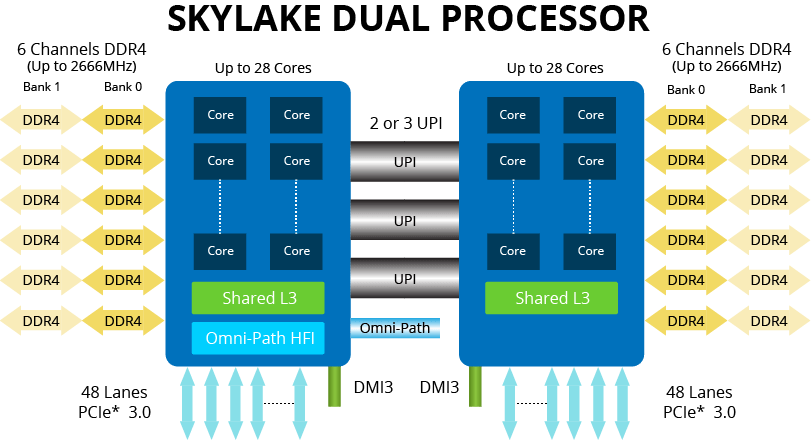
\includegraphics[width=10cm]{images/skylake_gold.png}
        \caption{\label{pic:skylake_gold} Architecture d'une plateforme avec deux processeurs Xeon Skylake (source \cite{Aspsys})}
    \end{figure}
    
    
    

    \subsubsection{Performances mémoires théoriques}
    %%%%%%%%%%%%%%%%%
        Le processeur Xeon Skylake 6148 possède 6 canaux mémoires pour accéder, dans notre expérimentation, à une mémoire DDR4-2666. En appliquant l'\autoref{eq:bw} nous obtenons une bande passante maximale de : $2666 \times 8 \times 6 = 128\ GB/s$. À cause de la loi de Little \cite{little2008little}, le processeur doit être capable de lancer plusieurs transactions simultanément (\textit{outstanding load}) pour saturer le bus mémoire et  atteindre cette performance. Nous avons montré dans la \autoref{sec:dml_saturation} que ce processeur nécessitait d'avoir au moins 15 coeurs actifs pour y parvenir.
        
    

    \subsubsection{Performances de calculs théoriques}
    %%%%%%%%%%%%%%%%%
        Le processeur étudié est un processeur superscalaire capable d'exécuter jusqu'à 4 instructions par cycle, dont deux opérations flottantes. Ces opérations pouvant être des instructions \gls{FMA} vectorielles de 512 bits. Il est donc possible de calculer sur chaque ALU, une multiplication et une addition par cycle sur 8 éléments simultanément. On peut ainsi calculer la performance crête de ce processeur en appliquant l'\autoref{eq:flops}. Suivant la fréquence utilisable par le processeur (dépendant de la température) la performance crête théorique, $FLOPS_{peak}$ est comprise entre $8 \times 2 \times 2 \times 1.6 \times 20 = 1024\ GFLOP/s$ et  $8 \times 2 \times 2 \times 2.2 \times 20 = 1408\ GFLOP/s$. 
        
        Cependant, pour comparer la performance de l'application avec ce résultat, il faut que la nature du code puisse utiliser des instructions FMA vectorisées. Il peut être intéressant de disposer d'une fourchette de performance lorsque la totalité du parallélisme est utilisée ou non. Quand le processeur n'utilise pas d'instruction AVX-512, le processeur est capable d'atteindre 3.1 GHz lorsque les 20 coeurs sont actifs. En reprenant l'\autoref{eq:flops}, la performance optimale d'une telle application serait: $FLOPS_{SISD} = 1 \times 1 \times 2 \times 3.1 \times 20 = 124 \ GFLOP/s$.
    

    \subsubsection{Équilibre arithmétique}
    %%%%%%%%%%%%%%%%%
        L'équilibre arithmétique du processeur permet d'évaluer s'il est approprié pour un code nécessitant une grande bande passante ou plutôt de bonnes performances de calculs. En réutilisant les deux caractéristiques précédemment calculées, on peut calculer $\text{EQUILIBRE}_{non\_avx}$ et $\text{EQUILIBRE}_{avx\_512}$ qui bornent la performance inférieure et supérieure de ce processeur. On obtient ainsi $\text{EQUILIBRE}_{non\_avx} = \frac{124}{128} = 0.97\ flop/byte$ et $EQUILIBRE_{avx\_512} = \frac{1408}{128} = 11\ \text{flopbyte}$. L'équilibre arithmétique est utilisé pour construire le modèle du Roofline présenté dans la \autoref{sec:roofline}.